\documentclass[tesi]{subfiles}
\IfEq{\jobname}{\detokenize{tesi}}{}{%
    \externaldocument{Chapter2}
\externaldocument{Chapter3}
\externaldocument{Chapter4}
\externaldocument{Chapter5}
\externaldocument{Chapter6}
}

\begin{document}
\chapter{Introduction}
\label{ch:Introduction}

The monitoring of the conditions of a road surface, such as the detection of anomalies associated with it, like potholes, bumps, joints, level passage, small covering defects, breaks, and theirs proper locations helps to improve road users' safety, from pedestrians to drivers and has a significant impact on the road maintenance. In fact, an adequate mapping of the road infrastructure can allow workers to intervene at the most critical points, or at the most disadvantaged sections of the road itself. For this reason, in order to offer a continuous efficient and up-to-date service, it is very important both to inform road users about the road surface quality and to obtain information from them.


The accurate evaluation of the quality of a road surface is a critical issue: transport system could become more efficient, comfortable and, most of all, safer. In fact, the presence of different types of anomalies on a road surface can make the transport-related energy efficiency worse, by increasing fuel consumption, a decay of suspensions and brakes. Crossing one of these anomalies both generates vibrations inside the tires' and suspensions' system, and affects the deformation of the tire, causing energy leaks and increasing rolling resistance. In addition, an increased risk of major damage to the vehicle (broken rims, tires puncture, or damage to the car body) can occur.

\clearpage
Road pavement monitoring is usually carried out through a variety of instruments, most of all various types of profilometers; however, especially in the most advanced cases, a profilography\footnote{The profilograph is a device used to measure pavement surface roughness} can be used, too.
Given the high cost of these instruments, the use of mobile technologies or cheap hardware sensors is widely adopted in this area, with the aim of providing to road users the opportunity to obtain real-time information about the road surface conditions and the traffic situation, or understand road accident cases promptly. All of that is made possible thanks to the hardware of these devices. In fact, if we mainly focus on smartphones and tablets, the majority of them uses a three-axis accelerometer to collect acceleration data, due to vehicle motion, and a GPS receiver to obtain location information of the current specific road segment.


This work focuses on the development of a system for the road surface conditions monitoring, that makes use of inertial measurement units (also known as \textbf{\textit{IMU}}), electronic hardware systems based on inertial sensors, such as the ones in our smartphones/tablets or Arduino devices, which have much lower prices than the standard instruments used for this task.
The system is based both on the reading of data collected through the smartphone, and on the post-processing elaborations of the GPS signal and acceleration data, (in which particular attention is given to vertical acceleration impulses, corresponding to \textbf{\textit{high-energy peaks}} and possibly representing an "\textit{anomaly}" of the road surface).
After all the data has been processed, the following benchmarks for the road surface conditions are extrapolated:
\begin{itemize}\label{it:indexes}
\item \textbf{IRI}: International Roughness Index: the international standard for road surface monitoring.
\item \textbf{Critical Points}: an index that locates and labels the most critical points on the road surface.
\item \textbf{Simple Acceleration Points}: an index able to interpret the variation of the acceleration signal on predetermined dimension segment of road travelled at different speeds.
\end{itemize}

The obtained results are shown on a web-site on an interactive map.

The \nameref{ch:Introduction} Chapter discusses the main instruments{\footnotesize (\ref{sc:Instruments})} used for the road surface monitoring, like profilometers{\footnotesize (\ref{ssc:profilometers}, page: \pageref{ssc:profilometers})}, and the reasons why this system was developed  {\footnotesize (\ref{sc:Motivation}, page: \pageref{sc:Motivation})}.


Subsequently, the Chapter\ref{ch:IRI} discusses about the \textit{IRI}, its history and its calculation.


Chapter\ref{ch:Inertial Measurement Unit}, talks about the Inertial Measurement Units (IMUs), specifying what they are, their functioning and physical principles, measurement accuracy, and how they are into smartphones.


Then, Chapter\ref{ch:Data Analysis} analyses  how these data can be processed in order to get road surface conditions, what these data represent and why both a data filtering, through the analysis of the filter types that can be used to improve the processing, and a Fourier Analysis are mandatory for that purpose.


Chapter\ref{ch:System Development} discusses the work that has been done, from the data-extraction through smartphones, to how the listed above indexes\ref{it:indexes}, whose elaboration is also explicated, are displayed on the map.
Eventually, the last Chapter\ref{ch:c_and_fw}, is focused on the obtained results and on possible future extensions.

	\section{Road surface monitoring instruments}\label{sc:Instruments}
It is possible to identify two main instruments' families for the measurement of the longitudinal road profile: \emph{static} and \emph{dynamic}. The first ones perform the measurement of road profile by points, thus in a statical manner, while the second ones through a dynamic method, due to their movements at high speeds; in fact, during the detection period, the vehicular traffic could be high, for this reason reaching high sampling rates could remove the noise of vehicle traffic, caused by the detection operation itself. However, over the years, it was preferred to distinguish these families as indirect and direct instruments.
The first ones are called \textit{Response Type Road Roughness Measuring Systems} \textbf{(RTRRMS)} and measure the \textit{"effect"}, produced by interaction vehicle-pavement, in kinematic terms (displacement, velocity or acceleration). The second ones, called \textbf{profilometers}, return the sampled road profile for points within a defined range, instead.

		\subsection{Profilometer}\label{ssc:profilometers}
Profilometers are capable of providing a digital profile of the road surface. Compared to RTRRMS, they can provide a more stable measure of road irregularities. In fact, the irregularity measures obtained by the RTRRMS systems are significantly affected by the inertial and mechanical characteristics of the vehicles on which they are mounted. However, even the measurement made by the profilometers represents an approximation of the actual road surface profile\cite{sayers1996interpretation}.

ISO-Standard\cite{iso_standard} identifies the following four fundamental properties to classify the profilometers:
\begin{enumerate}

\item \textbf{Instrument mobility}: For this property ISO-Standard\cite{iso_standard} provides four distinct classes.
\begin{description}
\item [Mobile, high speed]: referees to the vehicles equipped with profilometers which can be used at a test speed greater than or equal to $\num{60} \si{\km\per\hour}$.
\item [Mobile, low speed]: referees to the vehicles equipped with profilometers which can be used at a test speed smaller than to $\num{60} \si{\km\per\hour}$.
\item [Stationary in presence of traffic]: placed directly on the road surface at the point you want to detect.
\item [Stationary in absence of traffic]: cannot be moved quickly from a measurement site, e.g: during the measurement on a site, that one will be closed to the traffic.
\end{description}
\clearpage
\item \textbf{Detectable wavelength range:}\\ According to ISO-Standard\cite{iso_standard}, five ranges are indicated for this property, each-one distinguished by a letter:

\vspace{0.5cm}
\begin{table}[H]
\centering
    \begin{tabular}{ | l | l | l | l | l | l |}

    \hline
    Classes &\quad A &\quad B &\quad C &\quad D &\quad E \\ \hline
    Wavelength &	$ 0.05 \quad to \quad 0.16$&	$ 0.2 \quad to \quad 0.5$&		$0.63 \quad to \quad 2.0$&	$2.5 \quad to \quad 50$&	$63 \quad to \quad 500$\\
    \quad range &\quad $\si{\milli\meter}$ &\quad  $\si{\milli\meter}$ &\quad  $\si{\milli\meter}$ &\quad  $\si{\milli\meter}$ &\quad  $\si{\milli\meter}$ \\
\hline
    \end{tabular}
 \caption{Classification of profilometers according to ISO wavelength range}
 \label{table:iso_wave}
\end{table}

The wavelength allows understanding the type of a road pavement. In fact, the road surface, also called \textit{texture}, is divided among four distinct categories: microtexture, macrotexture, mega-texture and irregularity. Referring to the wavelength parameters shown in the table\ref{table:iso_wave}, the texture categories fall in this wavelength range\cite{sayers1996interpretation}:
\vspace{0.5cm}
\begin{table}[H]
\centering
    \begin{tabular}{ | l | l | l | l | l |}

    \hline
    Wavelength & \quad $\num{0.5} \thinspace \si{\milli\meter}$ & \quad $\num{50} \thinspace \si{\milli\meter}$ & \quad $\num{0.5}\thinspace \si{\meter}$ & $ > \num{0.5} \thinspace \si{\meter} $  \\ \hline
   \quad  Texture & microtexture& macrotexture &mega-texture &	irregularity \\

\hline
    \end{tabular}
 \caption{Texture class in function of wavelength}
\end{table}
A profilometer can detect one or more wavelength classes.
\clearpage
\item \textbf{Nature of instrument contact:}\label{ssc:Instrument_Contact}\leavevmode\\
According to the nature of the contact between the used instrument and the road surface, profilometers can be classified in:
\begin{itemize}
\item \textbf{Contact Devices:} the sensor that executes the reading during the measurement, establishes a real physical contact with the surface that is being investigated;

\item \textbf{Contactless Devices:} the reading sensors do not have physical contact with the road surface, therefore the height between the profilometer sensor and the road surface point is detected thanks to the projection on that point
\end{itemize}
The operating difference is substantial: the first has a direct contact with the road surface but it can not move at high speeds during the survey, which is the main prerogative of the second type, instead. 

For what concerns the accuracy of the measurement, the profilometers have been classified by the World Bank\cite{sayers1995calculation} as:
\begin{description}

	\item [Class 2]: devices that can make a random error during the survey;
	\item [Class 1]: very accurate devices: the possibility of measurements affected by a random error is extremely low.

\end{description}

\paragraph{Contact Profilometers}\leavevmode\\
The Walking Profiler or Dipstick\cite{little_book}, thanks to its precision in determining road profiles, falls into the Class 1 (high precision profilometers) of the World Bank rating\cite{sayers1995calculation}; it is even often used to calibrate other equipment.


\begin{figure}[H]
\centering
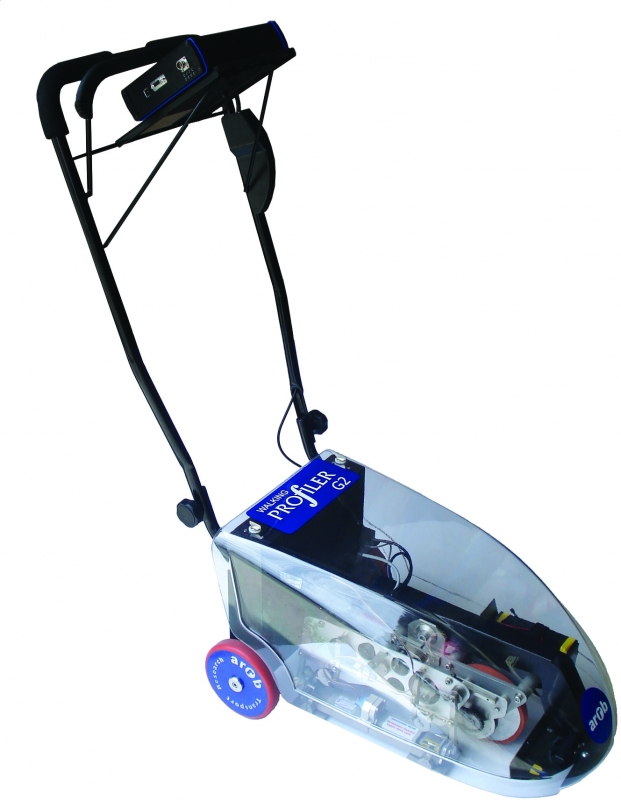
\includegraphics[scale=0.15]{Walking_Profiler}
\hspace{1.5cm}
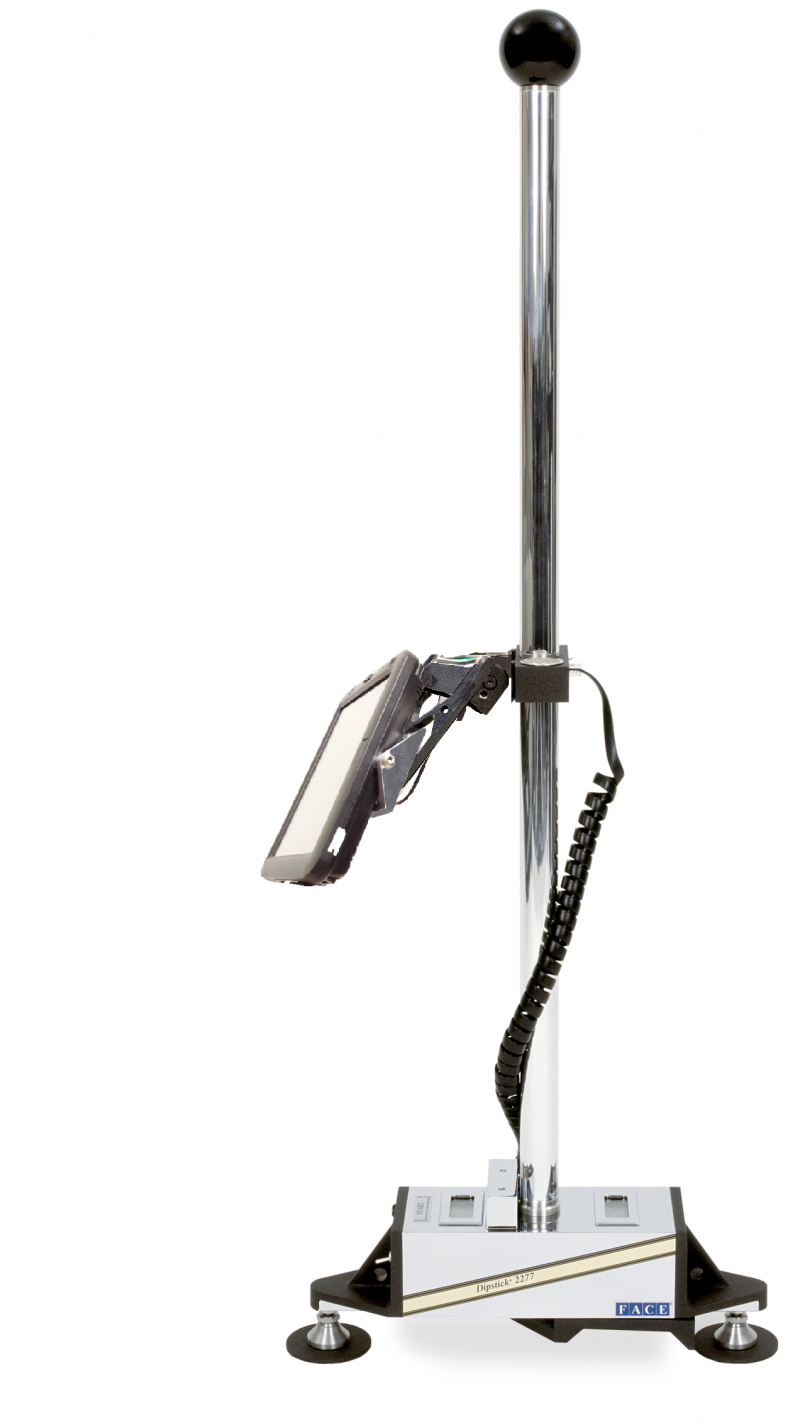
\includegraphics[scale=0.1]{Dipstick_Profiler}
\caption{Examples of Walking Profiler (left) and Dipstick Profiler (right).}
\label{fig:contact_profiler}
\end{figure}
\clearpage
\paragraph{Contactless Profilometers}\leavevmode\\  These profilometers are generally made up of one or more acoustic or electromagnetic sensors and mounted on a vehicle. Nowadays, laser is the most widely used sensors.
Laser sensors are extremely delicate and expensive. A single-sensor detection, however, only provides the relative dimension of the sensor over the road surface (height between the profilometer sensor and the road surface point), which is not sufficient to know the road profile. So, generally, in order to obtain a point of the road surface itself from a higher point over the vehicle, an accelerometer is placed on the sensor structure, which provides, through a double integration, the displacements of the sensor itself in correspondence of the road surface. The final goal of these profilometers is to extrapolate the IRI; that one, however, can not be detected only by one sensor, for the same principle of the IRI that discussed in the Chapter\ref{ch:IRI}.

\vspace{0.35cm}
\begin{figure}[H]
\centering
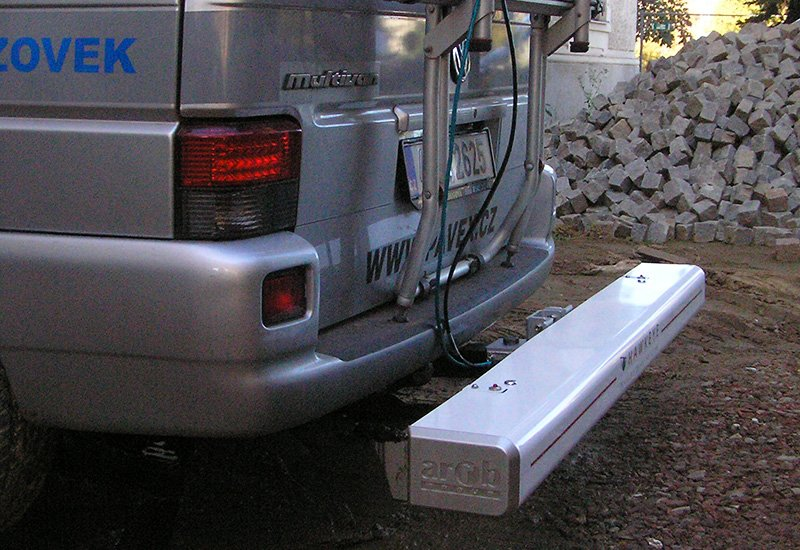
\includegraphics[scale=0.26]{High_Speed_Profilometer2}
\hspace{1cm}
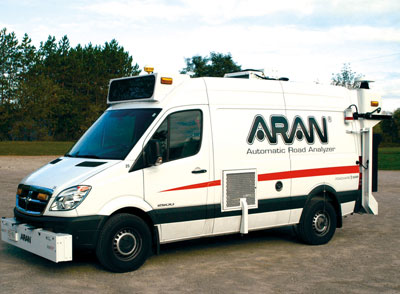
\includegraphics[scale=0.49]{High_Speed_Profilometer}
\caption{Examples of contactless profilometers mounted on the vehicle.}
\label{fig:contact_less_profiler}
\end{figure}

\item \textbf{Operating principle of the device:}\\ The easiest way to classify a profilometer is its internal operating principle.
According to this, four basic categories of profilometers were established\cite{measuring_equipment}.

\begin{description}

\item [Laser Profilometer] Makes use of an appropriate filtering, which can distinguish laser light from the ambient light with an excellent contrast. Generally, a laser profilometer consists of two fundamental components:
\begin{itemize}
\item Source of Emission
\item Capture-Transducer\footnote{A transducer is a device that converts one form of energy to another one.}
\end{itemize}
The operating principle of a laser profilometer is based on the optical principle of triangulation: the emission source projects a laser on the road surface, with a certain inclination angle to normal. The radius, diffused from the road surface, is received by the capture-transducer, which is also in an inclined position to receive the return signal. Then, the radius is transmitted through a lens to the transducer\cite{arnberg1991laser} (sensitive photo semiconductor). The capture-transducer source provides a signal $D$, as output data, proportional to the height $h$ (the distance between the laser incidence point on the road surface and the emission source).
\item [Stylus Profilometer] Represents the progenitor of all road surface monitoring instruments. It uses a pointed stylus, which touches the surface, and reads the small perceived irregularities, transforming them into other forms of energy. Then, an electric transducer transforms the mechanical movements of the needle into electric oscillations. These devices are equipped with a stylust needle, that is in a vertical position respect to the survey surface, which is lowered in order to physically touch the road surface. A transducer, mechanically connected to the needle, captures the magnitude of the vertical motion by transforming it into an electrical signal.
\item [Light Sectioning Profilometer:] Uses a light source to produce on the road surface a little line or a high band of light, with defined edges, on the road surface. A camera resumes this line of light with a certain inclination angle and with respect to the direction of the light. In the camera output, that consists of an x-z plane, the profile is represented by the contrast line between the illuminated area and the rest of the road surface. Generally, applying this kind of profilometers requires an high-resolution image management.
\item [Ultrasonic Profilometer:] Equipped with a mobile electro-acoustic sensor that emits and receives ultrasounds. These signals are first sent to the road surface, reflected and intercepted by a special microphone. The measurement is performed by considering the time between the transmission and the reception of the signal so that the distance between the ultrasonic source and the surveyed surface can be calculated\cite{little_book}.
\end{description}

\end{enumerate}
\clearpage
	\section{Motivation}\label{sc:Motivation}
As can be seen above, the monitoring of the conditions of a road surface is a critical issue, very useful for travellers and maintenance institutions.\\
With regards to travellers, it is very important to know the conditions of the road they will have to travel and their level of "comfort": inside the vehicle, passengers perceive a certain amount of vibrations, strongly dependent on the suspension system associated with vehicle in question.
To be able to improve the perceived comfort of road users is one of the aims of this work: travel comfortable road sections is better than travel the disadvantaged ones. Disadvantages roads, in fact, increase the risk of car damages and of fuel consumption (according to some studies, a good floor pavement could improve fuel consumption by $\displaystyle{\cong{2-6\%}}$\cite{jackson2011synthesis},\cite{jointeapa}).
Furthermore, in a constantly moving society like ours, the maintenance of roads becomes a central aspect of a municipal administration. The bad maintenance of the road surface has consequences not only on the safety and health of the drivers but also on the decor of the Commune itself. 
The investment that year after year the municipal authorities make for the viability are very low. And according to \cite{piemonte2013finanza}, only a few of the major Italian municipalities can exceed a spending average pro-capite of $\displaystyle{\euro 100,00}$.
So, having an effective monitoring system would help both drivers and organisations, thanks to a more efficient maintenance of the critical issues related to the roads.
However, the main matter is what tools have to be used in order to carry out the monitoring. In the previous section (\ref{ssc:profilometers}), in fact, we have analysed the profilometers, which are able to directly measure the quality of the road profile, but their cost is very high and only a very small number of people can make the surface monitoring. 
Thus, in this work only low-cost inertial measurement systems are used, such as the sensors of mobile devices, which, nowadays are owned by the majority of drivers, who could be able both to get almost effort-free road quality information and to actively participate in the collection of data.

\end{document}